\documentclass[10pt,a4paper,oneside,openany,noindent]{report}
\usepackage[utf8]{inputenc}
\usepackage{amsmath}
\usepackage{amsfonts}
\usepackage{amssymb}
\usepackage{graphicx}
\usepackage{subfigure}
\usepackage[margin=3cm]{geometry}
\usepackage{amssymb}
\usepackage{graphicx}
\setlength\parindent{0pt}
\usepackage[pagestyles]{titlesec}
%\titleformat{\chapter}[display]{\normalfont\bfseries}{}{0pt}{\Huge}
\newpagestyle{mystyle}
{\sethead[\thepage][][\chaptertitle]{}{}{\thepage}}
\pagestyle{mystyle}
\usepackage{algorithm}
\usepackage{algpseudocode}
\newcommand{\ph}{\hat{p}}
\newcommand{\direct}{x'|x}
\newcommand{\inverse}{x|x'}
\newcommand{\normal}[2]{\mathcal{N}\left(#1,#2\right)}
\newcommand{\pk}{\textbf{P}_k}
\newcommand{\pknew}{\textbf{P}_{k'}}
\newcommand{\eq}{\textbf{E}_q}
\newcommand{\eqnew}{\textbf{E}_{q'}}
\newcommand{\ak}{\textbf{a}_k}
\newcommand{\aknew}{\textbf{a}_{k'}}
\newcommand{\y}{\textbf{y}}
\newcommand{\bq}{\textbf{b}_q}
\newcommand{\bqnew}{\textbf{b}_{q'}}
\renewcommand{\eq}{\textbf{E}_q}
\newcommand{\ve}{\sigma_e^2}
\newcommand{\va}{\sigma_a^2}
\newcommand{\vb}{\sigma_b^2}
\newcommand{\la}{\lambda_a}
\newcommand{\lb}{\lambda_b}
\newcommand{\unif}{\mathcal{U}[0,1]}
\usepackage[]{frontespizio}
\begin{frontespizio}
\Universita{Università di Pisa}
\Universita {Università di Pisa}
\Logo [1.5cm]{4362142973_41e74dbc81_b.jpg}
\Facolta {DIPARTIMENTO DI INGEGNERIA DELL’INFORMAZIONE}
\Corso [Laurea]{Ingegneria robotica e dell’automazione}
\Annoaccademico{2015-2016}
\Titoletto {Progetto per il corso di identificazione dei sistemi incerti}
\Titolo {Identificazione di sistemi mediante modello NARMAX e
approccio bayesiano}
\Candidato [453645]{Giorgio Mirenda}
\Relatore {prof. Andrea Caiti}
\end{frontespizio}
\begin{document}
\hspace{1em}
\newpage

\chapter{Introduzione}
\section*{Premessa}

Questo relazione rappresenta il progetto per l'esame \emph{Identificazione dei Sistemi Incerti} del corso di studi di Ingegneria Robotica e dell'Automazione di Pisa uno studio critico dell'articolo di ricerca \textit{Computational system identification for Bayesian
NARMAX modelling} di Tara Baldacchino, Sean R. Anderson  e Visakan Kadirkamanathan.
\section*{Motivazioni}
Quando si vuole identificare un sistema dinamico bisogna
\begin{itemize}
\item stabilire la struttura del legge dinamica
\item stabilire il valore numerico delle costanti del modello
\end{itemize}
La prima richiesta consiste nel decidere il tipo e il numero di operazioni sui segnali di ingresso e di stato che sono in grado di riprodurre accettabilmente ( e possibilmente con una legge compatta) la dinamica del sistema.
La seconda richiesta consiste invece nel determinare il valore numerico dei parametri che intervengono.\\


I casi in cui è sufficiente una identificazione parametrica sono i casi in cui si ha già la struttura della legge. Per ottenere la legge (a meno del valore delle costanti) è necessario uno studio del sistema a partire dai principi primi che regolano tutti i fenomeni che sono coinvolti. In definitiva l'identificazione parametrica è sufficiente solo se sono verificate le seguenti condizioni
\begin{itemize}
\item è \textbf{possibile} ottenere una descrizione del sistema applicando i principi primi delle scienze
\item è \textbf{vantaggioso} ottenere una descrizione del sistema applicando i principi primi delle scienze (tempo speso, rischio di errori etc)
\item ci si accontenta della descrizione ottenuta applicando i principi primi delle scienze (rischio di tralasciare fenomeni importanti)
\item la complessità delle leggi che si ottengono applicando i principi primi delle scienze non è tale da renderle inutilizzabili
\end{itemize}

Quando una di queste condizioni non è soddisfatta è possibile inserire nel processo di identificazione anche la ricerca della struttura del modello.
A tale scopo si ipotizza una classe (abbastanza vasta) di strutture di modello
e si lascia al processo di identificazione l’onere di scegliere quella che maggiormente si adatta
alle misure e alle preferenze di modellazione. I metodi Bayesiani in particolare sono appropriati per la selezione dei
modelli perchè forniscono naturalmente (senza analisi aggiuntve) un contesto in cui
si quantifica l’incertezza associata all’identificazione. L’approccio bayesiano infatti, non fornisce una singola descrizione del sistema ma fornisce una distribuzione di
probabilità associata al set di modelli possibili. Dunque risolvere il problema di
inferenza bayesiana conduce a scelte più  ponderate rispetto alla semplice estrazione
del modello che si adatta meglio ai dati reali. Analizzando la distribuzione prodotta
si può per esempio individuare un modello poco meno accurato del migliore ma
preferirlo perchè meno complesso .\\
Nella seguente trattazione la classe di modelli scelta è quella dei nonlineari, auto-regressivi, a media mobile
con ingressi esogeni (NARMAX); essa è una popolare classe modelli ingresso-uscita
spesso usata nell’identificazione di sistemi non lineari in vari ambiti dell’ingegneria
(e non) poichè ha il pregio di produrre leggi compatte ma accurate.
Come si vedrà nei successivi capitoli, ciascun modello NARMAX può essere visto
come lo sviluppo su una opportuna base polinomiale della legge che
regola il sistema. Ciò che distingue un modello da un altro è il numero e l’insieme
dei termini presenti nello sviluppo.

La ricerca esaustiva tra tutte le possibili combinazioni di termini NARMAX è tuttavia quasi sempre computazionalmente improponibile , così si è puntato negli ultimi
anni a sviluppare metodi di campionamento efficaci che, avvalendosi di una catena
di Markov opportunamente costruita, esplorano in maniera non esaustiva l’insieme
dei modelli ottenendo comunque statistiche significative.
\chapter{Identificazione bayesiana e metodi
di campionamento Monte Carlo}
\section{Approccio Bayesiano per l’identificazione}
L’inferenza bayesiana è un approccio all’inferenza statistica in cui le probabilità
non sono interpretate come frequenze ma piuttosto come livelli di fiducia nel verificarsi di un dato evento. Il nome deriva dal teorema di Bayes, che costituisce il
fondamento di questo approccio. Gli statistici bayesiani sostengono che i metodi
dell’inferenza bayesiana rappresentano una formalizzazione del metodo scientifico,
che normalmente implica la raccolta di dati che avvalorano o confutano una data
ipotesi.
Queste caratteristiche rendono l’approccio bayesiano un utile ausilio per discriminare tra alternative in conflitto e dunque un ottimo strumento per l’identificazione
dei sistemi.
Il metodo usa una stima del grado di fiducia in una data ipotesi prima dell’osservazione
dei dati al fine di associare un valore numerico al grado di fiducia in quella stessa
ipotesi successivamente all’osservazione dei dati. Si supponga di voler identificare
un sistema scegliendo il più adatto in un insieme M di modelli.
Sia M una variabile aleatoria che rappresenta la legge che regola il vero sistema.
L’obiettivo dell’identificazione bayesiana è quello di calcolare per ogni $m\in M$ la
probabilità a posteriori
\begin{equation} P (M = m|Y )
\end{equation}
dunque complessivamente determinare la distribuzione della probabilità sull’insieme
dei modelli condizionatamente alle misure.\\
Una volta stimata la probabilità a posteriori, è possibile utilizzare il criterio MAP
\begin{equation}
m=arg \min_m P(M = m|Y )
\end{equation} oppure vari altri criteri per estrarre il modello da utilizzare.\\
La probabilità condizionata è stata definita in termini della probabilità congiunta e
marginale dei due eventi
\begin{equation}
P (M = m|Y ) =\frac{
P (M = m, Y )}{
P (Y )}
\end{equation}

la definizione corrisponde all’idea ragionevole che se fisso il valore di $Y$ allora
\begin{equation}
P (M = m|Y ) \propto P (M = m, Y )
\end{equation}

Avendo però ristretto l’insieme di supporto su cui è definita la metrica di probabilità (rispetto a quello della congiunta),
è necessario imporre che valgano ancora gli assiomi della probabilità, in particolare
chiamando k la costante di proporzionalità e integrando su tutti i casi possibili si ha
\begin{equation}\int P (M = m|Y )dm =
k \cdot \int P (M = m, Y )dm = k \cdot P (Y ) := 1\end{equation}
da cui si ricava il valore di k
\begin{equation}
k =\frac{1}{P(Y)}
\end{equation}
ottenendo la definizione di probabilità condizionata.
Scambiando i ruoli delle variabili aleatorie si ha anche che
\begin{equation}
P (Y |M = m) =\frac{
P (M = m, Y )}{
P (M = m)}
\end{equation}


dunque mettendo insieme le equazioni (2.3) e (2.7) si ottiene la formula di Bayes
\begin{equation}
P (M = m|Y ) =\frac{
P (Y |M = m)P (M = m)}{
P (Y )}
\end{equation}

usando il teorema della probabilità totale si può inoltre esprimere la costante al
denominatore in funzione delle quantità al numeratore ottenendo
\begin{equation}
P (M = m|Y ) =\frac{
P (Y |M = m)P (M = m)}{\int
P (Y |M = m)P (M = m)dm}
\end{equation}
Nei problemi di identificazione l’espressione della probabilità a posteriori è quasi
sempre impossibile da valutare analiticamente sopratutto per colpa dell’integrale al
denominatore che deve essere calcolato su tutti i possibili modelli; si ricorre quindi a
metodi numerici di tipo Monte Carlo basati sul campionamento della distribuzione.
Spesso risulta impossibile anche campionare direttamente la distribuzione e se ne
deve ottenere una stima accettando o scartando opportunamente i campioni estratti
da una distribuzione più semplice.
\section{Idea dei metodi Monte Carlo}
I metodi Monte Carlo sfruttano il seguente ragionamento: se si vuole  campionare una distribuzione con densità $p(x)$ (nel nostro caso la posterior sui modelli) si ha
\begin{equation}
p(x)=p(x)\otimes \delta(x)=\int_\xi p(\xi)\delta(x-\xi)d\xi
\end{equation}
se poi $p(x)$ è fattorizzabile come \begin{equation}
p(x)=q(x)g(x)
\end{equation}
tale che $q(x)$ sia una densità di probabilità ovvero
\begin{itemize}
\item $q(x)>0$ per ogni $m$
\item $\int_m q(x)=1$
\end{itemize} allora
\begin{equation}
p(x)=\int_\xi q(\xi)g(\xi)\delta(x-\xi)= E[g(Q)\delta(x-Q)]
\end{equation}
con $Q$ variabile aleatoria avente come densità $q(\cdot)$.
Usando uno stimatore si può approssimare il valore atteso come
\begin{equation}
E[g(Q)\delta(x-Q)]\simeq \frac{1}{N}\sum_{k=1}^N g(q_k)\delta(x-q_k)
\end{equation}
con $q_k\sim q(\cdot)$ campione estratto dalla distribuzione di densità di proposal $q(\cdot)$
In pratica si estraggono numerosi modelli da una distribuzione di proposal $q(\cdot)$,
e si costruisce un istogramma pesato con i pesi 
\begin{equation}
g(q_k)=\frac{p(q_k)}{q(q_k)}
\end{equation}
Si noti che nella formula dei pesi la desnsità  $p(\cdot)$ è solamente una funzione da valutare in uno specifico modello, cosa che quasi sempre è fattibile  perchè richiede una informazione che è locale nello spazio dei modelli, al contrario del problema di campionare direttamente la densità che richiederebbe una conoscenza della funzione su tutto lo spazio.\\
\section{Importance sampling: scelta della proposal}
In teoria le precedenti considerazioni sono già sufficienti per campionare la distribuzione, in pratica la scelta di una proposal opportuna è critica per l'accuratezza dell'algoritmo. Avendo a disposizione un tempo limitato, e quindi un numero limitato di campioni si otterrà solo una approssimazione della distribuzione cercata.\\
La proposal è determinante nell'imporre alcuni criteri di approssimazione\\
Partendo dal presupposto ovvio che non è possibile esplorare esaustivamente lo spazio dei modelli, bisogna fare delle assuzioni su quali regioni dello spazio dei modelli esplorare maggiormente (e quindi descrivere) e quali invece trascurare.\\
E' sensato disinteressarci delle regioni in cui i modelli hanno bassa probabilità.
Ai fini dell'identificazione, non ci interesserà mai confrontare due modelli con probabilità bassa. Si può benissimo sbagliare o ignorare il rapporto reciproco tra le loro probabilità per concentrarsi sulla descrizione delle regioni dove i modelli hanno probabilità più alta.
Questo induce a scegliere la proposal quanto più simile alla posterior, in modo da estrarre campioni prevalentemente dove la posterior è alta.
Tale criterio è detto di \emph{importance sampling}.\\ \\
Al limite se riuscissi ad essere sicuro che sto campionando da $q(\cdot)=p(\cdot)$ 
avrei che i pesi si ridurrebbero a
\begin{equation}
g(q_k)=\frac{p(q_k)}{q(q_k)}=\frac{p(q_k)}{p(q_k)}=1
\end{equation}
e dunque
\begin{equation}
p(x)\simeq \frac{1}{N}\sum_{k=1}^N \delta(x-q_k)
\end{equation}
Ovvero potrei avere una approssimazione di $p(\cdot)$ semplicemente valutando la frequenza relativa con cui è stato estratto $q_k=x$.
Attenzione, l'ipotesi di sapere che $q(\cdot)=p(\cdot)$ non vuol dire che conosco la forma della funzione su tutto lo spazio, ma solo che
\begin{itemize}
\item so valutare la funzione in un particolare modello
\item ho un metodo (anche indiretto) per campionare la funzione
\end{itemize}

Gli algoritmi Monte Carlo Markov Chain, infatti, ottengono i modelli $q_k$ 
come stati di una catena di Markov costruita sullo spazio dei modelli.\\ A  tale catena si chiede di avere come unica probabilità di regime proprio $p(\cdot)$.\vspace{2em}\\
Dopo un transitorio iniziale la catena finirà per campionare gli stati dalla distribuzione di regime $p(\cdot)$.
\chapter{Algoritmo Metropolis Hasting}
Supponiamo di voler estrarre campioni da una distribuzione p(m) nota, difficile da
campionare direttamente.
Si pu`o chiedere che la distribuzione obiettivo sia
distribuzione di regime di una catena di Markov. Una catena si dice ergodica se
dopo un certo tempo (transitorio iniziale) , essa converge all'unica distribuzione
di regime indipendentemente dalla distribuzione di partenza.
Le condizioni necessarie per l’ergodicit`a della catena sono:
\begin{itemize}
\item \textbf{irriducibilit`} : la probabilit`a di visitare ciascuno stato a partire da ciascuno
stato `e strettamente positiva
\item \textbf{aperiodicità} : una catena `e periodica se pu`o ritornare in un certo stato solo
a istanti multipli di un qualche intero maggiore di 1. Una catena `e aperiodica
se non `e periodica.
\end{itemize}

In poche parole, fissato un qualsiasi istante abbastanza grande e un qualsiasi stato,
deve essere possibile una storia temporale della catena che la porta a risiedere in
quello stato a quell’istante. La questione diventa quindi come scegliere il kernel
\begin{equation*}
s(x' |x) 
\end{equation*}
(probabilit`a di transizione dal vecchio stato m al nuovo stato m' ) della catena,
in modo che la catena sia ergodica e che la distribuzione di regime sia proprio p(m).
Una condizione sufficiente non necessaria `e che la distribuzione obiettivo soddisfi la
condizione di reversibilit`a

\begin{equation}
p(x)s(x' |x) = p(x')s(x|x' )
\end{equation}

L'operatore di transizione è quello che nelle catene a stato discreto e finito era rappresentato dalla matrice di transizione mentre nelle catene a stato continuo è il funzionale
\begin{equation}
Tr[\bullet]=\int \bullet(x)s(x'|x)dx
\end{equation}
Una  densit`a di probabilit`a $\ph$ `e detta stazionaria se `e autofunzione
dell’operatore di transizione della catena, ovvero\\
\begin{equation}
Tr[\ph]=\ph
\end{equation}
e semplice dimostrare che se vale la condizione di reversibilit`a allora la distribuzione
`e stazionaria infatti
\begin{equation*}
\begin{split}
Tr[\ph]=\int \ph(x)s(x'|x)dx=\int \ph(x')s(x|x')dx=\\
\ph(x')\int s(x|x')dx=\ph(x')\cdot 1=\ph(x')
\end{split}
\end{equation*}

Se si sceglie un kernel arbitrario uguale ad una probabilit`a di transizione facile
da campionare $s(\direct) = q(\direct) $ solitamente la condizione di reversibilit`a non `e
soddisfatta. Solitamente si ha uno sbilanciamento che significa che alcune transizioni
sono pi`u probabili in un certo verso.
\begin{equation}
\ph(x)s(\direct)>\ph(x')s(\inverse)
\end{equation}

In tal caso, viste le distribuzioni di partenza e la probabilit`a di transizione scelta `e
pi`u probabile osservare la transizione $x\rightarrow x'$ piuttosto che la transizione $x'\rightarrow x$
Si cerca quindi di ristabilire l’equilibrio scegliendo come kernel la probabilit`a di
transizione moltiplicata per un fattore correttivo 
\begin{equation}
q(\direct) = \gamma(\direct)q(\direct)
\end{equation}
In particolare si pu`o interpretare $\gamma(\direct)$ come la probabilit`a di accettare la mossa $x \rightarrow x'$. Imponendo quindi che valga


\begin{equation}
\ph(x)\gamma(\direct)q(\direct)=\ph(x')\gamma(\inverse)q(\inverse)
\end{equation}
si ricava
\begin{equation}
\frac{\gamma(\direct)}{\gamma(\inverse)}=\frac{\ph(x')q(\inverse)}{\ph(x)q(\direct)}
\end{equation}

Perch`e si abbia coerenza con la eq[CITARE EQUAZIONE] bisogna che il rapporto al membro sinistro sia minore di 1. In particolare si può scegliere

\begin{itemize}
\item $\gamma(\inverse)=1$ che equivale ad accettare tutte le transizioni $m' \rightarrow m$ che sono meno
frequenti
\item $\gamma(\direct)=min\left\lbrace 1,\frac{\ph(x')q(\inverse)}{\ph(x)q(\direct)}\right\rbrace$ fattore di riduzione delle transizioni pi`u frequenti
\end{itemize}
\newpage
 L'algoritmo MH è così definito\vspace{1em}\\
\hrule 
\textbf{Algoritmo} Metropolis Hastings
\hrule



\begin{algorithmic}
\State Inizializza  $X_0=x_0$
\For {$t=0,1,2\dots T$}
    \State $i\gets 0$

\State Estraggo la proposta per il nuovo stato $x^t \sim q(x^t |X_t)$
\State Calcolo la probabilità di accettare la mossa $\gamma(\direct)=min\left\lbrace 1,\frac{\ph(x^t)q(X_t | x^t)}{\ph(X_t)q(x^t|X_t  )}\right\rbrace$
\State Estraggo una variabile da una distribuzione uniforme $u\sim U(0,1)$
\If {$u \leq \gamma(x^t | X_t)$}
 \State La catena transita nel nuovo stato proposto $X_{t+1}=x^t$
\Else
\State La catena rimane nel vecchio stato $X_{t+1}=X_t$
\EndIf
\EndFor
\end{algorithmic}


\chapter{Reversible Jump Monte Carlo Markov Chain}
Nelle sezioni precedenti la transizione della catena associava (in maniera aleatoria)
uno stato di $M\subset \mathbb{R}^n$ ad uno stato di  $M'\subset \mathbb{R}^n$ .
Cosa succede se la transizione dovesse associare uno stato $M\subset \mathbb{R}^n$ ad uno stato
di $M\subset \mathbb{R}^m$ con $ m = n$?
La questione scaturisce dal fatto che per gli scopi dell’identificazione dei sistemi,
restringersi al caso $m = n$ `e molto limitativo e corrisponde a conoscere in partenza
il numero dei parametri da identificare.
Per i sistemi non lineari spesso si considerano modelli del sistema che sono sviluppi
polinomiali di equazioni alle differenze e si lascia all’algoritmo di identificazione
l’onere di determinare quali e quanti termini dello sviluppo includere.
In base al numero di termini scelti si avranno da scegliere anche altrettanti coeffici-
enti dello sviluppo.
Quando l’algoritmo suggerisca di aggiungere o eliminare uno (o pi`u) termini dello
sviluppo `e necessario aggiornare anche la dimensione del vettore dei coefficienti.
Ecco quindi che acquistano senso mosse che portano lo stato della catena da uno
spazio con una certa dimensionalit`a ad un’altro con dimensionalit`a diversa.
Si pensi quindi di enumerare le tipologie di modello (anche infinite), si avr`a che
l’insieme delle possibili strutture di modello `e rappresentabile come un insieme di
indici
\begin{equation*}
K=\left\lbrace 1,2,\dots k \right\rbrace
\end{equation*}
\chapter{Il modello}
\section{Modello Narmax}
Grazie all’uso di un modello esplicito di rumore, il modello NARMAX è in grado
di modellare l’effetto di rumori non bianchi, correlati a causa delle nonlinearità del
sistema.
Un sistema SISO tempo discreto può essere rappresentato da un modello NARMAX
descritto da
\begin{equation}
y_t=f(y_{t-1},\dots, y_{t-n_y},y_{t-1},\dots, y_{t-n_y},e_{t-1},\dots, e_{t-n_e})+e_t
\label{narmax}
\end{equation}
dove si assume che $f(\cdot)$ sia una funzione non lineare sconosciuta, $u_t\in\mathbb{R}$ e $y_t\in\mathbb{R}$ siano gli ingressi e uscite del sistema e $e_t\in\mathbb{R}$ denota un termine di rumore estratto dalla distribuzione normale $\normal{0}{\sigma_e^2}$.\\
Gli ordini della dinamica sono rispettivamente $n_u,n_y,n_e$.
Decomponiamo la funzione f (·) in una somma di funzioni di base polinomiali e
riesprimiamo la \ref{narmax} come combiaione di termini di processo e di rumore,
\begin{equation}
y_t=\sum_{j=1}^{M_p}\left(a_j y_{t-	\delta_{y,j}}^{k_{y,j}} u_{t-	\delta_{u,j}}^{k_{u,j}}\right)+
\sum_{j=1}^{M_e}\left(b_j y_{t-	\delta_{y,j}}^{k_{y,j}} u_{t-	\delta_{u,j}}^{k_{u,j}}
e_{t-	\delta_{e,j}}^{k_{e,j}}\right)+e_t
\end{equation}

dove il modello di processo è composto da $M_p$ monomi combinazione di soli termini
di uscita e di rumore e il modello di rumore è composto da $M_e$ monomi combinazione
di ingresso, uscita e rumore. Con $k_{y,j}$ , $k_{u,j}$ , $k_{e,j}\in N$ si indicano le potenze che compaiono nei monomi, con $\delta_{ y,j}$ , $\delta_{ e,j}\in \mathbb{N}-\{0\}$ e
$\delta_{ u,j}\in \mathbb{N}$ il ritardo delle varie grandezze.\\
Si ha quindi una forma pseudo-lineare dell'equazione di uscita
al passo attuale che per comodità è stata spezzata nella somma di due regressioni, una relativa al processo e una relativa al rumore
\begin{equation}
y_t=\phi_P(t,u,y)^T\ak+\phi_N(t,u,y,e)^T\cdot\bq+e_t
\end{equation}
In questa descrizione la mappa di uscita è lineare mentre tutta la non linearità è inserita negli elementi del regressore.\\
Dal modello si ottiene la formula dello stimatore
\begin{equation}
y_t=\phi_P(t,u,y)^T\cdot\ak+\phi_N(t,u,y,\epsilon(t,u,y,\ak,\bq))^T\cdot\bq
\end{equation} 

Si noti che nel modello teorico la non linearità è imputabile solo alla natura della funzione $f(\cdot)$ mentre nella espressione dello stimatore si aggiunge una ulteriore fonte di non linearità dovuta al fatto che la realizzazione del processo bianco $e(t)$ non è nota
e dunque si sostituisce con la realizzazione del residuo $\epsilon(t) $ che è funzione del vettore dei parametri.\\
Se si considera una finestra di campioni lunga $w$ per l'dentificazione si avranno a disposizione altrettante equazioni di regressione che per comodità possono essere impilate in una equazione vettoriale


\begin{equation}
\begin{pmatrix}
y(t) \\ 
y(t-1) \\ 
y(t-2) \\ 
\vdots \\ 
y(t-w+1)
\end{pmatrix} =\begin{pmatrix}
\phi_P(t,u,y)^T \\ 
\phi_P(t-1,u,y)^T \\ 
\phi_P(t-2,u,y)^T \\ 
\vdots \\ 
\phi_P(t-w+1,u,y)^T
\end{pmatrix}\ak+\begin{pmatrix}
\phi_N(t,u,y,e)^T \\ 
\phi_N(t-1,u,y,e)^T \\ 
\phi_N(t-2,u,y,e)^T \\ 
\vdots \\ 
\phi_N(t-w+1,u,y,e)^T
\end{pmatrix}\bq+\begin{pmatrix}
e(t) \\ 
e(t-1) \\ 
e(t-2) \\ 
\vdots \\ 
e(t-w+1)
\end{pmatrix}
\end{equation}
indicata compattamente come
\begin{equation}
\y=\pk\ak+\eq\bq+e \label{reg}
\end{equation}

\section{Densità di probabilità a posteriori del modello}
Dal teorema di Bayes
\begin{equation}
p(k, q, \pk , \eq, \ak , \bq |\y) \propto p(\y|k, q, \pk ,\eq , \ak, \bq , \ve )p(k, q, \pk, \eq,\ak,\bq ) \label{post}
\end{equation}
\subsection{Likehood}
Se il rumore è gaussiano a media nulla anche la verosimiglianza è una gaussiana, funzione del vettore dei residui, di stessa varianza. Infatti come si deduce dall’equazione
di regressione (\ref{reg}) si ha
\begin{equation}
p(\y|k,\,\pk,eq,\ak,\bq,\ve)=p(\pk\ak+\eq\bq+\epsilon|k,q,\pk,\eq,\ak,\bq,\ve)=p(\epsilon|k,q,\pk,\eq,\ak,\bq,\ve)
\end{equation}
e supponendo di aver identificato correttamente i termini e i parametri in modo tale
da avere come errore residuo (ineliminabile) il rumore di misura si ha
\begin{equation}
p(\textbf{e}|k, q, \pk , \eq , \ak , \bq , \ve ) = p(\epsilon |k, q, \pk , \eq , \ak , \bq , \ve )=\frac{1}{\sqrt{2\pi\ve}^N}exp\left(-\frac{1}{2\ve}\epsilon^T\epsilon\right)
\end{equation}
dunque in definitiva
\begin{equation}
p(\y|k,\,\pk,eq,\ak,\bq,\ve)=\frac{1}{\sqrt{2\pi\ve}^N}exp\left(-\frac{1}{2\ve}\epsilon^T\epsilon\right)
\end{equation}
con
\begin{equation}
\epsilon=\y-\pk\ak-\eq\bq
\end{equation}
\section{Scelta delle distribuzioni a priori e iperparametri}
In assenza di preferenze, la scelta delle distribuzioni a priori solitamente ricade su
distribuzioni poco informative ovvero densità con un supporto ampio e varianza
grande.\\
Per aumentare la flessibilità si adotta una struttura gerarchica in cui gli stessi
parametri delle distribuzioni a priori sono a loro volta realizzazioni di variabili aleatorie. Per convenienza si sceglie di rappresentare i parametri con una distribuzione a
prori coniugata della likehood.
\section{Il concetto di distribuzioni coniugate}
Sia X una variabile che modella il sistema estratta da una distribuzione $p(X=x|\zeta)$.
Supponiamo cioè che il profilo della distribuzione sia dipendente dal parametro $\zeta$.\\
Per la variabile aleatoria $X$ la $p(X|\zeta)$ rappresenta la probabilità a priori rispetto ai dati.\\
Se si concentra l'attenzione sul parametro e si assume che anche esso abbia natura aleatoria la stessa $p(X|\zeta)$ rappresenta invece la likehood  del parametro $\zeta$ rispetto alle realizzazioni della $X$. 
Per la variabile che rappreseta il parametro vale quindi la regola di Bayes
\begin{equation}
p(\zeta|X)\propto p(X|\zeta)p(\zeta)
\end{equation}
La distribuzione $p(X|\zeta)$ è quindi un operatore che mappa una distribuzione in un'altra. E’ possibile per tale operatore trovare una sorta di \emph{autofunzione}, nel senso
 lato di distribuzione appartenente a una certa famiglia (normale, uniforme, poisson etc ) che viene mappata dall’operatore in un’altra funzione ancora appartenete
alla medesima famiglia.
Data una certa likehood le sue \emph{autofunzioni} in questo senso, vengono dette distribuzioni coniugate.

Se i prior sono scelti tra le distribuzioni coniugate, quando (mediante l’applicazione
dell’operatore likehood) evolvono non cambiano la forma d’onda ma solo i parametri
che la descrivono. Quindi la descrizione di una dinamica su uno spazio funzionale a
infinite dimensioni viene rappresentata dalla dinamica in uno spazio il cui numero di
dimensioni è finito e ridotto. (Ad esempio l’evoluzione di una gaussiana può essere
rappresentata concisamente dall’evoluzione del suo valor medio e della sua varianza).\\
Se  i prior non sono scelti tra le distribuzioni coniugate, invece, ad ogni applicazione
dell’operatore likehood cambia l’intera forma d’onda della distribuzione diventando
impossibile da descrivere analiticamente.
\subsection{Probabilità del modello a priori}
Modificando leggermente la (\ref{post}) per tenere conto anche degli iperparametri (descritti nel dettaglio in questa sezione) si ha
\begin{equation}
p(k,q,\pk,eq,\ak,\bq,\va,\vb,\la,\lb|\y)\propto
p(\y|k,q,\pk,ak,\bq,ve)
p(k,q,\pk,\eq,\ak,\bq,\va,\vb,\la,\lb)
\end{equation}
fattorizzabile come
\begin{align}
p(k,q,\pk,eq,\ak,\bq,\va,\vb,\la,\lb|\y)= & p(\ak|\pk,k,\va)p(k|\la)p(\pk)p(\la)p(\va)\times \nonumber\\
& p(\bq|\eq,q,\vb)p(q|\lb)p(\eq)p(\lb)p(\vb)
\end{align}
Di seguito vediamo nel dettaglio come sono state modellate le distribuzioni a priori
\subsection*{Vettore dei parametri dei termini di modello}
Il vettore di parametri $\ak$ si assume distribuito come una gaussiana multidimensionale isotropica a media nulla ovvero
\begin{equation}
p(\ak|k, \pk , \va ) = p(\ak |k, \va ) \sim \normal{\textbf{0}}{\va\textbf{I}}
\end{equation}
Questa scelta implica che la varianza della gaussiana sia distribuita come una gamma
inversa in modo da essere coniugata. La distribuzione gamma inversa è definita come
segue
\begin{equation}
\mathcal{I}\mathcal{G}(x|\alpha,\beta)= x^{-\alpha-1}\exp\left(-\frac{\beta}{x}\right)
\end{equation}
Di seguito si prova che la distribuzione gamma inversa è effettivamente coniugata
della gaussiana per l’iperparametro varianza\\
\textit{Proof.} è sufficiente applicare la regola di Bayes e ottenere ancora una gamma inversa
\begin{align*}
p(\va|k,\ak) & \propto p(\ak,k,\va)\cdot p(\va)\\
			 &\propto   \frac{1}{\sqrt{\va}^k}exp\left(\frac{-\ak^T\ak}{2\va}\right)\sigma_a^{2(-\alpha_a-1)}exp\left(-\frac{\beta_a}{\va}\right)\\
			 &\propto  \sigma_a^{2(-\alpha_a-1-\frac{1}{2}k)}exp\left(-\frac{\beta_a+\frac{1}{2}\ak^T\ak}{\va}\right) \\ 
			 &\propto   \sigma_a^{2(-\alpha_a-1-\frac{1}{2}k)}exp\left(-\frac{\beta_a+\frac{1}{2}\ak^T\ak}{\va}\right) \\
			 &\propto \mathcal{I}\mathcal{G}(\va|\alpha+\frac{1}{2}k,\beta_a+\frac{1}{2}\ak^T\ak)	
\end{align*}
 \begin{flushright}
 $\square$
 \end{flushright}

 \subsection*{Vettore dei parametri dei termini di rumore}
 La modellazione del vettore dei parametri dei termini di rumore è analoga a quella
trattata nella sottosezione precedente. Il vettore di parametri $\bq$ si assume distribuito come una gaussiana multidimensionale isotropica a media nulla
\begin{equation}
p(\bq |k, \eq , \vb ) = p(\bq |q, \vb ) \sim \normal{\textbf{0}}{\vb\textbf{I}}
\end{equation}

Questa scelta implica che la varianza della gaussiana sia distribuita come una gamma
inversa in modo da essere coniugata. Con dimostrazione del tutto analoga alla
sezione precedente si dimostra che la varianza della gaussiana deve essere una gamma
inversa.
\begin{align*}
p(\vb)=\mathcal{I}\mathcal{G}(\vb|\alpha_b,\beta_b)\Rightarrow
p(\vb|q,\bq) & \propto p(\bq,q,\vb)\cdot p(\vb)\\
	 &\propto \mathcal{I}\mathcal{G}(\vb|\alpha_b+\frac{1}{2}q,\beta_b+\frac{1}{2}\bq^T\bq)	
\end{align*}

\subsection*{Numero di termini di processo}
La probabilità a priori del numero di termini di processo è rappresentata da una
distribuzione di Poisson troncata, il parametro $\la$.
\begin{equation}
p(k|\la)=\frac{\frac{\la^k}{k!}}{\sum_{i=0}^N\frac{\la^i}{i!}}
\end{equation}
Con N numero massimo di termini di processo.
Questo tipo di distribuzione è più indicato rispetto ad una distribuzione uniforme,
perchè l’iperparametro $\la$ può essere interpretato come il numero medio di termini
ipotizzando un numero di termini possibili sufficientemente alto infatti
\begin{equation}
\mathbb{E}[k|\la]=\frac{\sum_{k=0}^Nk\frac{\la^k}{k!}}{\sum_{i=0}^N\frac{\la^i}{i!}}=\frac{\sum_{k=1}^Nk\frac{\la^k}{k!}}{\sum_{i=0}^N\frac{\la^i}{i!}}=\la\frac{\sum_{j=0}^{N-1}k\frac{\la^j}{j!}}{\sum_{i=0}^N\frac{\la^i}{i!}}=
\la\frac{\sum_{j=0}^{N-1}k\frac{\la^j}{j!}}{\sum_{i=0}^{N-1}\frac{\la^i}{i!}+\frac{\la^N}{N!}}=\la\frac{1}{1+\frac{\frac{\la^N}{N!}}{\sum_{i=0}^{N-1}\frac{\la^i}{i!}}}
\end{equation}
si noti che
\begin{equation}
\lim_{N\rightarrow\infty}\frac{\frac{\la^N}{N!}}{\sum_{i=0}^{N-1}\frac{\la^i}{i!}}=0
\end{equation}
L’iperparametro $\la$ è estratto da una distribuzione gamma
\begin{equation}
p(\la)=\mathcal{G}\mathcal{A}(\la|\alpha_{\la},\beta_{la})=\la^{(\alpha_{\la}-1)}exp\left(-\frac{\la}{\beta_{\la}}\right)
\end{equation}
Di seguito dimostro che la distribuzione gamma è coniugata per il parametro della
poisson
\textit{Proof.}
\begin{align*}
p(\la|k)&\propto p(k|\la)p(\la)\\
&\frac{\la^k}{k!}\la^{(\alpha_{\la}-1)}exp\left(-\frac{\la}{\beta_{\la}}\right)\\
&\propto\frac{1}{k!}\mathcal{G}\mathcal{A}(\la|\alpha_{\la}+k,\beta_{\la})
\end{align*}
 \begin{flushright}
 $\square$
 \end{flushright}
 \subsection*{Numero di termini di rumore}
 Analogamente a quanto detto nella sezione precedente, il numero dei termini di
rumore è modellato come una variabile aleatoria Poisson troncata
\begin{equation}
p(q|\lb)=\frac{\frac{\lb^q}{q!}}{\sum_{i=0}^N\frac{\lb^i}{i!}}
\end{equation}
e il suo iperparametro $\lb$ è modellato come una variabile aleatoria gamma-distribuita
\begin{equation}
p(\lb)=\mathcal{G}\mathcal{A}(\lb|\alpha_{\lb}.\beta_{\lb})=\lb^{(\alpha_{\lb}-1)}exp\left(-\frac{\lb}{\beta_{\la}}\right)
\end{equation}
\subsection*{Matrice di regressione dei termini di processo e di
rumore}
La matrice di regressione dei termini è considerata una va aleatoria uniformemente
distribuita in modo che nessun termine di modello nè di rumore sia, a priori delle
misure, più probabile di altri
\begin{equation}
p(\pk)\propto 1
\end{equation}
\begin{equation}
p(\eq )\propto 1
\end{equation}

\chapter{Algoritmo RJMCMC per
l’identificazione di modelli
NARMAX}

 L'algoritmo MH è così definito\vspace{1em}\\
\hrule 
\textbf{Algorithm} RJMCMC for NARMAX identification
\hrule



\begin{algorithmic}
\State fissa i parametri di tuning $c$ e $\ve$
\State inizializza$\left(k^{(0)},q^{(0)},\pk^{(0)},\eq^{(0)},\ak^{(0)},\bq^{(0)},\la^{(0)},\lb^{(0)},\sigma_a^{(0)},\sigma_b^{(0)}\right)$
\vspace{2em}
\For {$i=1:N_{\text{iter}}$}
    \State Estrai $z_k\sim \unif$
    \If {$z_k\leq B_k^{(i)}$}
    \State Effettua la mossa di nascita (Algoritmo 1)
    \ElsIf{$z_k\leq B_k^{(i)}+D_k{(i)}$}
\State Effettua mossa di morte (Algoritmo 2)
\Else
\State Aggiorna i parametri (Algoritmo 3)
\State Aggiorna la varianza dei  parametri
\EndIf
\State Estrai $\lb^{(i)}\sim p(\lb|q^{(i)})$
\vspace{2em}
\If {$i>$}
    \State Estrai $z_q\sim \unif$
    \If {$z_q\leq B_q^{(i)}$}
    \State Effettua la mossa di nascita (Algoritmo 1)
    \ElsIf{$z_k\leq B_q^{(i)}+D_q{(i)}$}
\State Effettua mossa di morte (Algoritmo 2)
\Else
\State Aggiorna i parametri (Algoritmo 3)
\State Aggiorna la varianza dei  parametri
\EndIf
\EndIf
\vspace{2em}
\State Calcola l'errore residuo $\epsilon^{(i)}=\y-\pk^{(i)}\ak^{(i)}-\eq^{(i)}\bq^{(i)}$:assumilo come stima del segnale di  rumore
\State Aggiornamento di $\eq^{(i)}$ in base alla nuova stima
\EndFor
\end{algorithmic}

L’algoritmo parte con l’inizializzazione di parametri e iperparametri: solitamente si
inizia con un modello vuoto ovvero con nessun termine (di rumore e di processo),
le matrici di regressione sono in tal caso (per convenzione) una singola colonna
di elementi nulli e il vettore dei parametri è lo scalare nullo. Gli iperparametri
delle poisson troncate vengono inizializzati a quello che ci si aspetta essere il numero medio di termini nello sviluppo, mentre le varianze dei coefficienti vengono
inizializzate ad un valore non piccolo in modo da avere inizialmente dei prior molto
dispersi e quindi poco informativi. L’inizializzazione di questi parametri non è critica perchè essi verranno aggiornati con l’evoluzione della catena e si adatteranno al
valore più appropriato. La varianza $\ve$ del rumore bianco invece viene inizializzata
e non viene più aggiornata, tale parametro rappresenta infatti un parametro di tuning dell’algoritmo essendo in qualche modo una metrica di affidabilità delle misure,
è sensato dunque che esso influisca direttamente sulla probabilità di accettazione
delle mosse: abbassare tale parametro equivale a ritenere l’incertezza bassa quindi
il rapporto di accettazione sarà più selettivo e le mosse proposte verranno scartate
più frequentemente.
L’algoritmo prevede un numero fissato a priori di iterazioni. In corrispondenza di
ciascuna iterazione la catena di Markov andrà a risiedere in uno stato che rappresenta un modello del sistema. L’assunzione di \textbf{ergodicità} permette di ricostruire la probabilità che la catena risieda in un particolare stato a partire dal
numero di iterazioni medio in cui la catena risiede in quello stato. E’ necessario però
adottare due accorgimenti:
\begin{itemize}
\item il numero di iterazioni deve essere abbastanza elevato da fare in modo che valga
con buona approssimazione l’ipotesi di ergodicità. Se le statistiche si raccolgono su poche iterazioni le probabilità che si ottengono sono molto influenzate
dalla particolare realizzazione della catena.
\item il numero medio di iterazioni in corrispondenza del quale la catena risiede in
un particolare stato deve essere calcolato escludendo le prime iterazioni della
catena (il cosiddetto periodo di burnin), questo perchè
le prime iterazioni sono fortemente influenzate dalla particolare inizializzazione
dei parametri e dello stato.
\end{itemize}
Nel contesto della singola iterazione eseguono due algoritmi analoghi: l’evoluzione
del modello di processo e l’evoluzione del modello di rumore.
Entrambi prevedono una fase in cui si seleziona la tipologia di mossa, una fase in cui
si effettua la mossa scelta e infine una fase in cui si estrae un nuovo iperparametro
per il numero medio di termini.
Dopo che hanno eseguito questi algritmi si calcola il nuovo errore di regressione come
differenza tra le uscite misurate del sistema e le uscite predette dal modello.
Assumendo poi che il modello attuale sia capace di descrivere esattamente l’uscita
misurata, si considera l’errore di regressione come se fosse la realizzazione del rumore gaussiano bianco e si aggiorna la matrice di regressione del rumore.
Per ottenere l’output dell’identificazione basta tenere in memoria (a partire da
quando si ritiene esaurito il transitorio iniziale) i modelli visitati dalla catena e
costruire progressivamente gli istogrammi sul numero di termini, sull’identificativo
dei termini e sul coefficiente associato a ciascun identificativo dei termini. Di seguito
si illustrano le tipologie di mossa previste, il meccanismo di scelta della tipologia di
mossa e nelle sezioni seguenti si entra nel dettaglio di come vengono effettuate le
mosse.
\subsection{Tipologia di mosse}
Le mosse che modificano lo stato della catena, nell’algoritmo dell’articolo sono:
\begin{itemize}
\item Nascita:\\
Viene selezionato un nuovo termine tra quelli rimasti e viene inserito nello
sviluppo polinomiale, togliendolo dall’insieme dei termini disponibili per una
futura mossa di nascita. Il numero di termini del modello passa da $k$ a $k' =
k + 1$.\\
I coefficienti dello sviluppo vengono estratti nuovamente
\item Morte:\\
Viene selezionato un nuovo termine tra quelli presenti nello sviluppo polino-
miale e viene eliminato reinserendolo nell’insieme dei termini disponibili per
una successiva mossa di nascita. Il numero di termini del modello passa da $k$
a $k' = k-1$\\
I coefficienti dello sviluppo vengono estratti nuovamente
\item Aggiornamento:\\
Non si ha cambio di dimensionalità $k'=k$
Vengono solamente cambiati i coefficienti dello sviluppo e la varianza della
distribuzione da cui sono estratti.
\end{itemize}
Mosse analoghe sono previste per i termini di rumore.
Ad ogni iterazione della catena,viene estratta una delle tre mosse.\\
La mossa di nascita viene estratta con probabilità $B_k$ dove
\begin{equation}
B_k=\begin{cases}
1 & k=0\\
0 & k=M_p\\
c\cdot\min\left\lbrace 1,\frac{p(k+1|\la}{p(k|\la)}\right\rbrace & \text{altrimenti}
\end{cases}
\end{equation}
La mossa di morte viene estratta con probabilità
\begin{equation}
D_k=\begin{cases}
0 & k=0\\
c\cdot\min\left\lbrace 1,\frac{p(k-1|\la}{p(k|\la)}\right\rbrace & \text{altrimenti}
\end{cases}
\end{equation}
La mossa di aggiornamento viene estratta con probabilità
\begin{equation}
U_k=1-B_k-D_k
\end{equation}
La costante c serve per regolare la frequenza relativa tra mosse che cambiano la
dimensionalità (morte e nascita) e la mossa di aggiornamento.\\
La scelta delle probabilità di nascita e di morte garantisce che
\begin{equation}
B_k p(k|\lambda)=D_{k+1}  p(k+1|\lambda) \label{equilibr_dimensi}
\end{equation}

La (\ref{equilibr_dimensi}) è una equazione di equilibrio bilanciato per il solo numero di termini.
Questo vuol dire che se si avesse solo l’informazione del numero di termini (nessuna
informazione sui coefficienti o sul tipo di termini,quindi nessuna idea sull’errore di
regressione) la probabilità del numero di termini convergerebbe alla distribuzione a
priori. In realtà nelle prossime sezioni si aggiungerà un meccanismo di accettazione
o rifiuto delle mosse che va di fatto ad alterare la probabilità di regime del numero
di termini in modo da tenere conto anche dell’errore di regressione (informazione
delle misure) piuttosto che delle sole informazioni a priori.
\subsection{Estrazione di una tipologia di mossa}
L’estrazione della tipologia di mosse deve avvenire con le probabilità $B_k$ , $U_k$ , $D_k$
calcolate come descritto nella sezione precedente. Un modo semplice per imporre
tale probabilità è la seguente:\\

\begin{algorithmic}
\State Estrai $z_k\in\unif$
\If {$z_k\leq B_k$}
\State Effettuare la mossa di nascita
\ElsIf {$B_k<z_k\leq B_k+D_k$}
\State Effettuare la mossa di morte
\Else
\State Effettuare la mossa di aggiornamento
\EndIf
\end{algorithmic}
per mostrare che si ottengono effettivamente le probabilità cercate basta integrare
tra gli estremi opportuni la ddp della variabile uniforme che è un l’impulso
rettangolare
\begin{equation}
P\left(0<z_k\leq B_k^{(i)}\right)=\int_0^{B_k^{(i)}}rect(z-0.5)dz=\int_0^{B_k^{(i)}}dz={B_k^{(i)}}
\end{equation}
\begin{equation}
P\left(B_k^{(i)}<z_k\leq B_k^{(i)}+D_k^{(i)}\right)=\int_{B_k^{(i)}}^{B_k^{(i)}+D_k^{(i)}}rect(z-0.5)dz=\int_0^{D_k^{(i)}}dz={D_k^{(i)}}
\end{equation}

\begin{equation}
P\left(B_k^{(i)}+D_k^{(i)}<z_k\leq 1 \right)=\int_{B_k^{(i)}+D_k^{(i)}}^{1}rect(z-0.5)dz=\int_{B_k^{(i)}+D_k^{(i)}}^{1}dz=1-{B_k^{(i)}}-{D_k^{(i)}}=U_k^{(i)}
\end{equation}
con
\begin{equation}
rect(z)=\begin{cases}
0 & abs(z)\leq 0.5\\
1 & abs(z)>0.5 
\end{cases}
\end{equation}

\section{Mossa di nascita}
\hrule 
\textbf{Algorithm 3} Mossa di nacita
\hrule

\begin{algorithmic}
\State All'iterazione $i$ estrai casualmente un termine di processo $p^{(i)}$ quelli non ancora selezionati
\State Calcola la quantità $r_a$
\State Calcola il rapporto di accettazione della mossa di nascita $\gamma_{\textit{birth}}^{(k)}$
\State Estrai $z_b\in\unif$
\If{$z_b\geq\gamma_{\textit{birth}}^{(k)}$}
\State k:=k+1
\State $ \mathcal{P}_k^{(i)}= \mathcal{P}_k^{(i-1)}\cup \{p^{(i)}\} $
\State aggiornare i parametri con il valor medio della proposal $\ak:=\mu_{a,k'}$
\Else
\State Aggiorna i parametri usando (l'algoritmo 3)
\State Aggiorna la varianza $\va$
\EndIf
\end{algorithmic}
\hrule
\vspace{2em}


Il termine da aggiungere nello sviluppo viene scelto casualmente (con probabilità
uniforme) tra i termini disponibili ovvero non già presenti nell’attuale modello.
Una volta scelto il termine candidato è necessario decidere se accettare o meno la
mossa di nascita alla maniera di RJMCMC, in modo da far convergere la catena
all’equilibrio rappresentato dalla posterior dei modelli.\\
\vspace{2em}
In particolare si accetta la mossa di nascita con probabilità
\begin{equation}
\gamma_{\textit{birth}}^{(k)}=min\{1,r_a\}
\end{equation}
a tal fine viene estratto un numero da una distribuzione $z_b\in\unif$,si accetta la
mossa se $z_b\geq \gamma_{\textit{birth}}^{(k)}$ birth e si rifiuta se $z_b> \gamma_{\textit{birth}}^{(k)}$ .
Il rapporto di accettazione $r_a$ viene calcolato come
\begin{equation}
r_a=\frac{\ph(x')g'(u')}{\ph(x)g(u)}\left\vert\frac{\partial(\theta_{k'},u')}{\partial(\theta_{k},u)}\right\vert
\end{equation}
si ha che $\ph$(x ) è la distribuzione target della catena (la posterior) calcolata nel
nuovo stato . Visto che il modello di rumore e gli iperparametri si tengono fissi
durante la transizione si ha che
\begin{equation}
\ph(x')=p(k',\pknew,\aknew|\y,\la,\va)
\end{equation}

si noti che le variabili $k,\pk$, identificano complessivamente una particolare struttura
del modello che è fissata dalla tipologia di mossa, non si ha quindi da effettuare particolari richieste per essi mentre bisogna imporre la condizione di \textit{ dimension matching}
sui vettori dei parametri e delle variabili ausiliarie chiedendo che la trasformazione\\
\begin{equation}
(\ak,u)\rightarrow(\aknew,u')
\end{equation}
sia un diffeomorfismo, si scelgono quindi le variabili ausiliarie in modo che valga.
\begin{equation}
dim(\ak)+dim(u)=dim(\aknew)+dim(u')
\end{equation}
Una possibile scelta è $u = \ak$ e $u' =\aknew$. Il jacobiano del cambio di variabili è
\begin{equation}
\left\vert\frac{\partial(\ak,\aknew)}{\partial(\aknew,\ak)}\right\vert=
\left\vert\frac{\partial\begin{bmatrix}
0 & I_k \\ 
I_{k'} & 0
\end{bmatrix}
 \begin{bmatrix}
\aknew \\ 
\ak
\end{bmatrix} }{\partial(\aknew,\ak)}\right\vert
=\begin{vmatrix}
0 & I_k \\ 
I_{k'} & 0
\end{vmatrix}=|-1|=1
\end{equation}
dunque
\begin{equation}
r_a=\frac{p(k',\pknew,\aknew |\y,\la,\va)p(\ak|\y,k',\pknew,\va)}{p(k,\pk,\ak |\y,\la,\va)p(\aknew|\y,k',\pknew,\va)}
\end{equation}
Per semplificare $r_a$ e evitare di estrarre un vettore $\ak$ dalla distribuzione si può far
uso dell’equazione del candidato di Besag (Si veda in seguito).\\
Con l’equazione di Besag ed alcuni passaggi algebrici, l’espressione di $r_a$ si semplifica
\begin{equation}
r_a=\frac{p(k',\pknew|\y,\la,\va)}{p(k,\pk|\y,\la,\va)}=\frac{\sigma_a^{-k'}\sqrt{det(\canew)}
exp(\mez\muanew^T\invcanew\muanew)p(k'|\la)}{\sigma_a^{-k}\sqrt{det(\canew)}
exp(\mez\mua^T\invca\mua)p(k|\la)} \label{ra}
\end{equation}
dove

\begin{equation}
\ca=\sigma_e^{-2}\pk^T\pk+\sigma_a^{-2}I_k
\end{equation}
\begin{equation}
\mu_{a,k}=\sigma_e^{-2}\ca(\pk^T(\y-\eq\bq) \label{mu}
\end{equation}
Dunque se la mossa di nascita viene accettata, il termine proposto viene aggiunto
allo sviluppo incrementando di conseguenza il conteggio del numero di termini. I
coefficienti dello sviluppo vengono aggiornati con gli elementi del vettore valor medio
calcolato mediante la (\ref{mu})
Se invece la mossa viene rifiutata i termini dello sviluppo rimangono gli stessi mentre
si aggiornano i coefficienti dello sviluppo e viene estratta una nuova varianza per i
coefficienti.
\subsection{Mossa di morte}
\hrule 
\textbf{Algorithm 3} Mossa di morte
\hrule

\begin{algorithmic}
\State All'iterazione $i$ estrai casualmente un termine di processo $p^{(i)}$ da quelli attualmente  selezionati
\State Calcola la quantità $r_a$
\State Calcola il rapporto di accettazione della mossa di morte $\gamma_{\textit{death}}^{(k)}$
\State Estrai $z_d\in\unif$
\If{$z_d\geq\gamma_{\textit{death}}^{(k)}$}
\State k:=k-1
\State $ \mathcal{P}_k^{(i)}= \mathcal{P}_k^{(i-1)}- \{p^{(i)}\} $
\State aggiornare i parametri con il valor medio della proposal $\ak:=\mu_{a,k'}$
\Else
\State Aggiorna i parametri usando (l'algoritmo 3)
\State Aggiorna la varianza $\va$
\EndIf
\end{algorithmic}
\hrule
\vspace{2em}
Il termine da eliminare dallo sviluppo viene scelto casualmente (con probabilità
uniforme) tra i termini già presenti nell’attuale modello
Una volta scelto il termine candidato è necessario decidere se accettare o meno la
mossa di morte alla maniera di RJMCMC, in modo da far convergere la catena
all’equilibrio rappresentato dalla posterior dei modelli
In particolare si accetta la mossa di morte con probabilità
\begin{equation}
\gamma_{\textit{birth}}^{(k)}=min\left\lbrace 1,r_a\right\rbrace
\end{equation}
Con $r_a$ ottenuto mediante l’equazione (\ref{ra})
Per imporre la probabilità di accettazione viene estratto un numero da una distribuzione
 $z_d\in\unif$,si accetta la
mossa se $z_d\geq \gamma_{\textit{death}}^{(k)}$ birth e si rifiuta se $z_b> \gamma_{\textit{death}}^{(k)}$ .
Dunque se la mossa di morte viene accettata, il termine proposto viene eliminato
dallo sviluppo e reinserito tra i termini disponibili per le future mosse di nascita,viene
decrementato di conseguenza il conteggio del numero di termini. I coefficienti dello
sviluppo vengono aggiornati con gli elementi del vettore valor medio calcolato mediante la (\ref{mu}).
Se invece la mossa viene rifiutata i termini dello sviluppo rimangono gli stessi mentre
si aggiornano i coefficienti dello sviluppo e viene estratta una nuova varianza per i
coefficienti.
\subsection{Aggiornamento dei parametri}
\hrule 
\textbf{Algorithm 5} Aggiornamento dei parametri
\hrule

\begin{algorithmic}
\For{m=1:k}
\State Estrarre un candidato $\hat{a_m}^{(i)}\sim\mathcal{N}(a_m^{(i-1)},C_{m,m})$ per $a_m^{(i)}$ 
\State Porre $a_{-m}^{(i)}=a_{-m}^{(i-1)}$
\State Calcolare la probabilità di accettazione
\[
\alpha(\hat{a_m}^{(i)}|a_m^{(i-1)})=\min\left\lbrace 1, \frac{p(\hat{a_m}^{(i)}|a_{-m}^{(i-1)},\y) q(a_{-m}^{(i-1)}|a^{(i)})}{p(a_m^{(i-1)}|a_{-m}^{(i-1)},\y)q(\hat{a_m}^{(i)}|a^{(i-1)}} \right\rbrace
\]
\State $z\sim\unif$
\If {$z\geq \alpha(\hat{a_m}^{(i)}|a_m^{(i-1)})$}
\State $a_m^{(i)}=\hat{a}_m^{(i-1)}$
\Else
\State $a_m^{(i)}=a_m^{(i-1)}$
\EndIf
\EndFor
\end{algorithmic}
L’aggiornamento dei parametri viene fatto campionando la ddp a posteriori dei
parametri stessi
\begin{equation}
p(\ak|\y,k,\pk,\eq,\va)
\end{equation}
che usando Bayes può essere espressa come

\begin{equation}
p(\ak|\y,k,\pk,eq,\va)\propto p(\y|\pk,\eq,\ak,\bq,\ve)p(\ak|k,\va)\propto exp\left\lbrace- \frac{\epsilon^T\epsilon}{2\ve}\right\rbrace p(\ak|k,\va)
\end{equation}
con
\begin{equation}
\epsilon=\y-\pk\ak-\eq\bq
\end{equation}
e
\begin{equation}
p(\ak|k,\va)=\normal{\textbf{0}}{\va \mathbb{I}}
\end{equation}
I parametri sono aggiornati sequenzialmente usando un algoritmo di tipo MH che,
invece di campionare la posterior multivriata la approssima campionando la probabilità dei singoli coefficienti condizionate rispetto agli altri. Dato però che anche le
singole probabilità condizionate non sono semplici da campionare, si ricorre ad una
densità di proposal scelta come gaussiana di varianza $C_{m,m}$ (l’ m-esimo elemento
della diagonale della matrice $C_{a,k}$ ) e valor medio il vecchio coefficiente $a_m^{(i-1)}$ . Il
coefficiente proposto viene accettato (sostituito al posto del corrispondente vecchio
coefficiente) con una probabilità che è calcolata alla maniera di MH.
\begin{equation}
\alpha(\hat{a}_m^{(i)}|a_m^{(i-1)})=min\left\lbrace 1,\frac{p(\hat{a}_m^{(i)}|a_{-m}^{(i-1)},\y)q(a_{-m}^{(i-1)}|a^{(i)})}
{p(a_{-m}^{(i-1)}|a_{-m}^{(i-1)},\y)q(\hat{a}_m^{(i)}|a^{(i)})})\right\rbrace
\end{equation}
Nella espressione sopra si è omesso il simbolo k che indica la struttura di modello a
cui si riferisce il vettore di coefficienti. Se non c’è il pedice si indica tutto il vettore
dei coefficienti. Il simbolo di accento circonflesso indica l’elemento estratto dalla
proposal. Il pedice m indica che si sta parlando dell’m-esimo elemento del vettore,
il pedice -m indica il vettore di tutti i coefficienti escluso l’m-esimo. L’apice indica
l’iterazione di RJMCMC in cui è stato calcolato il termine: quelli che hanno apice
(i-1) sono i vecchi coefficienti mentre quelli con apice (i) sono quelli calcolati
nell’attuale iterazione. Con probabilità $1-\alpha(\hat{a}_m^{(i)})|a_m^{(i-1)}$ il coefficiente proposto
viene rifiutato e rimane pari al vecchio valore.

\section{Equazione del candidato di Besag}
La formula utilizzata per semplificare l’espressione del rapporto $r_a$ è detta formula
del candidato. Il nome le è stato attribuito dal professore e statista Julian Ernst
Besag a fine anni ’80 quando era docente alla University of Durham (Inghilterra). Egli riporta
la formula in un articolo spiegando di averla letta (senza dimostrazione) nello svolgimento di un esame da parte di uno studente del quale però non ricordava più il
nome. Non sapremo quindi mai chi fu il primo ad averla pensata. Nonostante anche
Besag tralasci la dimostrazione della formula, questa non è complessa e deriva in
sostanza dalla formula di Bayes applicata opportunamente alla densità congiunta
delle tre variabili in gioco.
Si supponga di aver raccolto un vettore di misurazioni x ,sia $\theta$ un vettore di parametri
del modello, ci si chiede quale sia la densità di probabilità di una nuova misura z
condizionata alle vecchie misure ovvero $p(z|x)$

tesi:
\begin{equation}
p(z|x)=\frac{p(z|\theta)p(\theta|x)}{p(\theta|z,x)}
\end{equation}
dimostrazione: Dalla definizione di ddp condizionata
\begin{equation}
p(z|x)=\frac{p(z,x)}{p(x)}
\end{equation}
Per sviluppare il numeratore è necessario prima di tutto dimostrare un passaggio
intermedio Si consideri la tautologia
\begin{equation}
p(x,\theta,z)=p(z,\theta,z)
\end{equation}
dove ciascun membro è la ddp congiunta delle tre variabili in esame. utilizzando la
definizione di ddp condizionata
\begin{equation}
p(\theta|z, x)p(z, x) = p(z, x|\theta)p(\theta)
\end{equation}
utilizzando l’indipendenza della nuova misura rispetto alle precedenti
\begin{equation}
p(\theta|z, x)p(z, x) = p(z|\theta)p(x|\theta)p(\theta)
\end{equation}
da cui
\begin{equation}
p(z,x)=\frac{p(z|\theta)p(x|\theta)p(\theta)
}{p(\theta|z,x)}
\end{equation}
utilizzando Bayes
\begin{equation}
p(z|x)=\frac{p(z|\theta)\frac{p(\theta|x)p(x)}{p(\theta)}}{p(\theta|z,x)p(x)}
\end{equation}
Da cui la tesi
\begin{equation}
p(z|x)=\frac{p(z|\theta)p(\theta|x)}{p(\theta|z,x)}
\end{equation}
ponendo
\begin{equation}
z:=(z,\pk)
\end{equation}
\begin{equation}
x:=(y,\la,\va)
\end{equation}
\begin{equation}
\theta:=(\ak)
\end{equation}
si ha
\begin{equation}
p(k,\pk|y,\la,\va)=\frac{p(k,\pk|\ak)p(\ak|y,\la,\va)}{p(\ak|k,\pk,y\la,\va)}
\end{equation}
usando la definizione di probabilità condizionata si nota come il prodotto al numeratore non sia altro che la probabilità congiunta delle variabili k, $\pk$ e $\ak$ , ottenendo
quindi
\begin{equation}
p(k,\pk|y,\la,\va)=\frac{p(k,\pk,\ak|y,\la,\va)}{p(\ak|y,k',\pknew,\va)}
\end{equation}
Da cui la semplificazione per l'acceptance ratio
\begin{equation}
r_a=\frac{p(k',\pknew|\y,\la,\va)}{p(k,\pk|\y,\la,\va)}
\end{equation}.
Dovrò quindi calcolare
\begin{equation}
p(k,\pk|\y,\la,\va)
\end{equation}
che può essere ottenuta come probabilità marginale
\begin{equation}
p(k,\pk|\y,\la,\va)=\int p(k,\pk,\ak|y\la,\va)d\ak
\end{equation}
Usando Bayes l'integranda diventa
\begin{align*}
& \frac{1}{p(\y)}p(\y|k,\pk,\ak,\la,\va,q,\eq,\lb,\bq,\ve)p(k,\pk,\ak|\la,\va)\\
=&\frac{1}{p(\y)}p(k|\la)p(\pk)p(\y|k,\pk,\ak,\la,q,\eq,\lb,\bq,\ve)p(ak|k,\va)\\
=&\frac{1}{p(\y)}p(k|\la)p(\pk)\normal{\pk\ak+\eq\bq}{\ve I_k}\normal{0}{\va I_k}\\
=& \mathcal{K}\cdot exp[ \mez \sigma_e^{-2}(\y-\eq\bq)^{T}(\y-\eq\bq)+\mez \sigma_e^{-2}\ak^{T}(2\pk^{T}\y-2\pk^T\eq\bq)-\\
&\mez\ak^T(\sigma_e^{-2}\pk^T\pk+\sigma_a^{-2}I_k)\ak ]
\end{align*}
con
\begin{equation}
\mathcal{K}=\frac{1}{p(y)}\frac{\sigma_e^{-N}}{\sqrt{2\pi}^N}\frac{\sigma_a^{-k}}{\sqrt{2\pi}^k}p(k|\la)p(\pk)
\end{equation}
Si moltiplichi e si divida per $\mathcal{N}({\ak |\mu,C})$
\begin{align*}
&\mathcal{K}\sqrt{(2\pi)^k det(C)} exp[ \mez \sigma_e^{-2}(\y-\eq\bq)^{T}(\y-\eq\bq)+\mez \sigma_e^{-2}\ak^{T}(2\pk^{T}\y-2\pk^T\eq\bq)-\\
&\mez\ak^T(\sigma_e^{-2}\pk^T\pk+\sigma_a^{-2}I_k)\ak+\mez(\ak-\mu)^TC^{-1}(\ak-\mu) ]\mathcal{N}(\ak|\mu,C)
\end{align*}
con semplici manipolazioni algebriche si ottiene
\begin{align*}
\mathcal{K}\sqrt{(2\pi)^k det(C)}
exp[\mez\sigma_e^{-2}(\y-\eq\bq)^{T}(\y-\eq\bq)-\mez\ak^T(\sigma_e^{-2}\pk^T\pk+\sigma_a^{-2} I_k-\\C^{-1})\ak+\ak^T(\sigma_e^{-2}\pk^T\y-\sigma_e^{-2}\pk^T\eq\bq-C^{-1}\mu)+\mez(\mu^TC^{-1}\mu)]\mathcal{N}(\ak |\mu, C)
\end{align*}
annullando l’espressione tra parentesi che costituisce la matrice della forma quadratica in a $\ak$ e l’espressione tra parentesi che costituisce la matrice che moltiplica  $\ak^T$ ,si ricava l’espressione per la media e la covarianza
\begin{equation}
C=\sigma_e^{-2}\pk^T\pk+\sigma_a^{-2} I_k
\end{equation}
\begin{equation}
\mu=\sigma_e^{-2} C\pk^T(\y-\eq\bq)
\end{equation}
grazie al quale l’integranda si semplifica in modo tale che tutta la dipendenza da $\ak$ sia attribuita alla gaussiana di parametri $\mu$ e $C$.\\
Calcolando l’integrale si ottiene
\begin{align*}
p(k,\pk | \y,\la,\va)&=\sqrt{(2\pi)^k det(C)}\mathcal{K}p(k |\la)p(\pk) exp[\mez\sigma_e^{-2}(\y-\eq\bq)^{T}(\y-\eq\bq)+\\&\mez(\mu^T C^{-1}\mu)\int \mathcal{N}(\ak|\mu,C)d\ak\\
&=p(k|\la)p(\pk)\sqrt{(2\pi)^k det(C)}\mathcal{K}\cdot exp[\mez \sigma_e^{-2}(\y-\eq\bq)^{T}(\y-\eq\bq)+\mez(\mu^T C^{-1}\mu)]
\end{align*}
da cui
\begin{equation}
r_a=\frac{p(k',\pknew|\y,\la,\va)}{p(k,\pk|\y,\la,\va)}=\frac{\sigma_a^{-k'}\sqrt{det(\canew)}
exp(\mez\muanew^T\invcanew\muanew)p(k'|\la)}{\sigma_a^{-k}\sqrt{det(\canew)}
exp(\mez\mua^T\invca\mua)p(k|\la)}
\end{equation}

Nell'articolo originale non è esplicitato come comportarsi quando si propone una transizione da o verso $k=0$.\\
Per rispondere bisogna notare che nel caso di modello vuoto si può pensare di avere matrice di regressione nulla e vettore dei parametri arbitrario, per convenzione si sceglierà $\ak=0$. Il valore di $\ak$ è allora deterministico.\\
Tornando ad esprimere l'integranda si ha
\begin{align*}
=&\frac{1}{p(\y)}p(k=0|\la)p(\pk)p(\y|k,\pk,\ak,\la,q,\eq,\lb,\bq,\ve)p(ak|k,\va)\\
=&\frac{1}{p(\y)}p(k=0|\la)p(\pk)\normal{\pk\ak+\eq\bq}{\ve I_k}\delta(\ak-0)\\
=&\frac{1}{p(\y)}p(k=0|\la)p(\pk)\normal{\eq\bq}{\ve I_k}\delta(\ak-0)\\
\end{align*}
e dunque marginalizzando si ottiene
\begin{align*}
=&\frac{1}{p(\y)}p(k=0|\la)p(\pk)\normal{\eq\bq}{\ve I_k}\int\delta(\ak-0)d\ak\\
=&\frac{1}{p(\y)}p(k=0|\la)p(\pk)\normal{\eq\bq}{\ve I_k}\\
\end{align*}
Il resto è analogo. Se si vuole per esempio calcolare il rapporto di accettazione $r_a(k=1\rightarrow k=0)$ si ottiene
\begin{align*}
\frac{p(k=0,\pk | \y,\la,\va)}{p(k=1,\pk | \y,\la,\va)}&=\\
&\frac{\frac{1}{p(\y)}p(k=0|\la)p(\pk)\normal{\eq\bq}{\ve I_k}}{p(k=1|\la)p(\pk)\sqrt{(2\pi)^k det(C_{k,\ak})}\mathcal{K}\cdot exp[\mez \sigma_e^{-2}(\y-\eq\bq)^{T}(\y-\eq\bq)+\mez(\mu_{k,\ak}^T C_{k,\ak}^{-1}\mu_{k,\ak})]}
\end{align*}
e semplificando
\begin{align*}
\frac{p(k=0,\pknew | \y,\la,\va)}{p(k=1,\pk | \y,\la,\va)}&=\frac{p(k=0|\la)}{p(k=1|\la)\sqrt{det(C_{k,\ak})}\sigma_a^{-k}\cdot exp[\mez(\mu_{k,\ak}^T C_{k,\ak}^{-1}\mu_{k,\ak})]}\\&=
\frac{1}{\la\sqrt{det(C_{k,\ak})}\sigma_a^{-k}\cdot exp[\mez(\mu_{k,\ak}^T C_{k,\ak}^{-1}\mu_{k,\ak})]}
\end{align*}
per il passaggio inverso si ha invece
\begin{align*}
\frac{p(k=1,\pknew | \y,\la,\va)}{p(k=0,\pk | \y,\la,\va)}=\frac{\la\sqrt{det(C_{k',\aknew})}\sigma_a^{-k'}\cdot exp[\mez(\mu_{k',\aknew}^T C_{k',\aknew}^{-1}\mu_{k',\aknew})]}{1}
\end{align*}
\chapter{Tuning degli iperparametri}
La distribuzione gamma ha il seguente valor medio
\begin{equation}
\mathbb{E}[\mathcal{G}\mathcal{A}(\alpha,\beta)]=\frac{\alpha}{\beta}
\end{equation}
e la seguente varianza
\begin{equation}
\mathbb{V}ar[\mathcal{G}\mathcal{A}(\alpha,\beta)]=\frac{\alpha}{\beta^2}
\end{equation}
mentre la distribuzione gamma inversa ha per valor medio
\begin{equation}
\mathbb{E}[\mathcal{I}\mathcal{G}(\alpha,\beta)]=\frac{\beta}{\alpha-1}
\end{equation}
e varianza
\begin{equation}
\mathbb{V}ar[\mathcal{I}\mathcal{G}(\alpha,\beta)]=\frac{\beta^2}{(\alpha-1)^2(\alpha-2)}
\end{equation}
\chapter{Risultati del lavoro}
\section*{Correzione di una svista nell'articolo originale}
Nell'articolo \emph{Computational system identification for Bayesian
NARMAX modelling} sul quale si è basata la mia implementazione, in particolare nell'equazione (42) è stato omesso un segno meno.
L'errore sembra essere sfuggito alla revisione.
La likehood corretta è infatti
\[p(y|P_k,E_q,a_k,b_q,\sigma_e^2)=\prod_{t=1}^N \exp \left(-\frac{\epsilon_t^2}{2\sigma_e^2}\right)\]
Questo errore è intuibile dato che il residuo è distribuito come una Gaussiana,
inoltre la likehood, nonostante sia scritta sotto forma di produttoria,dovrebbe essere la stessa dall'equazione (5) dove si legge il segno meno. In ogni caso per avvalorare la mia correzione ho  fatto un test sull'algoritmo in un caso banale. Questo test mi serve anche a validare il codice in un caso di studio estremamente semplificato .
\\
In questo caso il modello era fissato ad una costante scalare e venivano effettuate solo mosse di aggiornamento dei coefficienti.
Il vero modello era
\[y(t)=0.2+e(t)\]
con
\[\sigma_e= 0.07\]
Il modello con cui era stata inizializzata lidentificazione è
\[y(t)=0.4+e(t)\]
Ho graficato l'andamento del coefficiente identificato in funzione del numero di iterazioni
Di seguito l'andamento del coeffciente provando come dice l'articolo con il segno più.\\
\begin{figure}[ht]
\centering
\begin{minipage}[b]{0.45\linewidth}
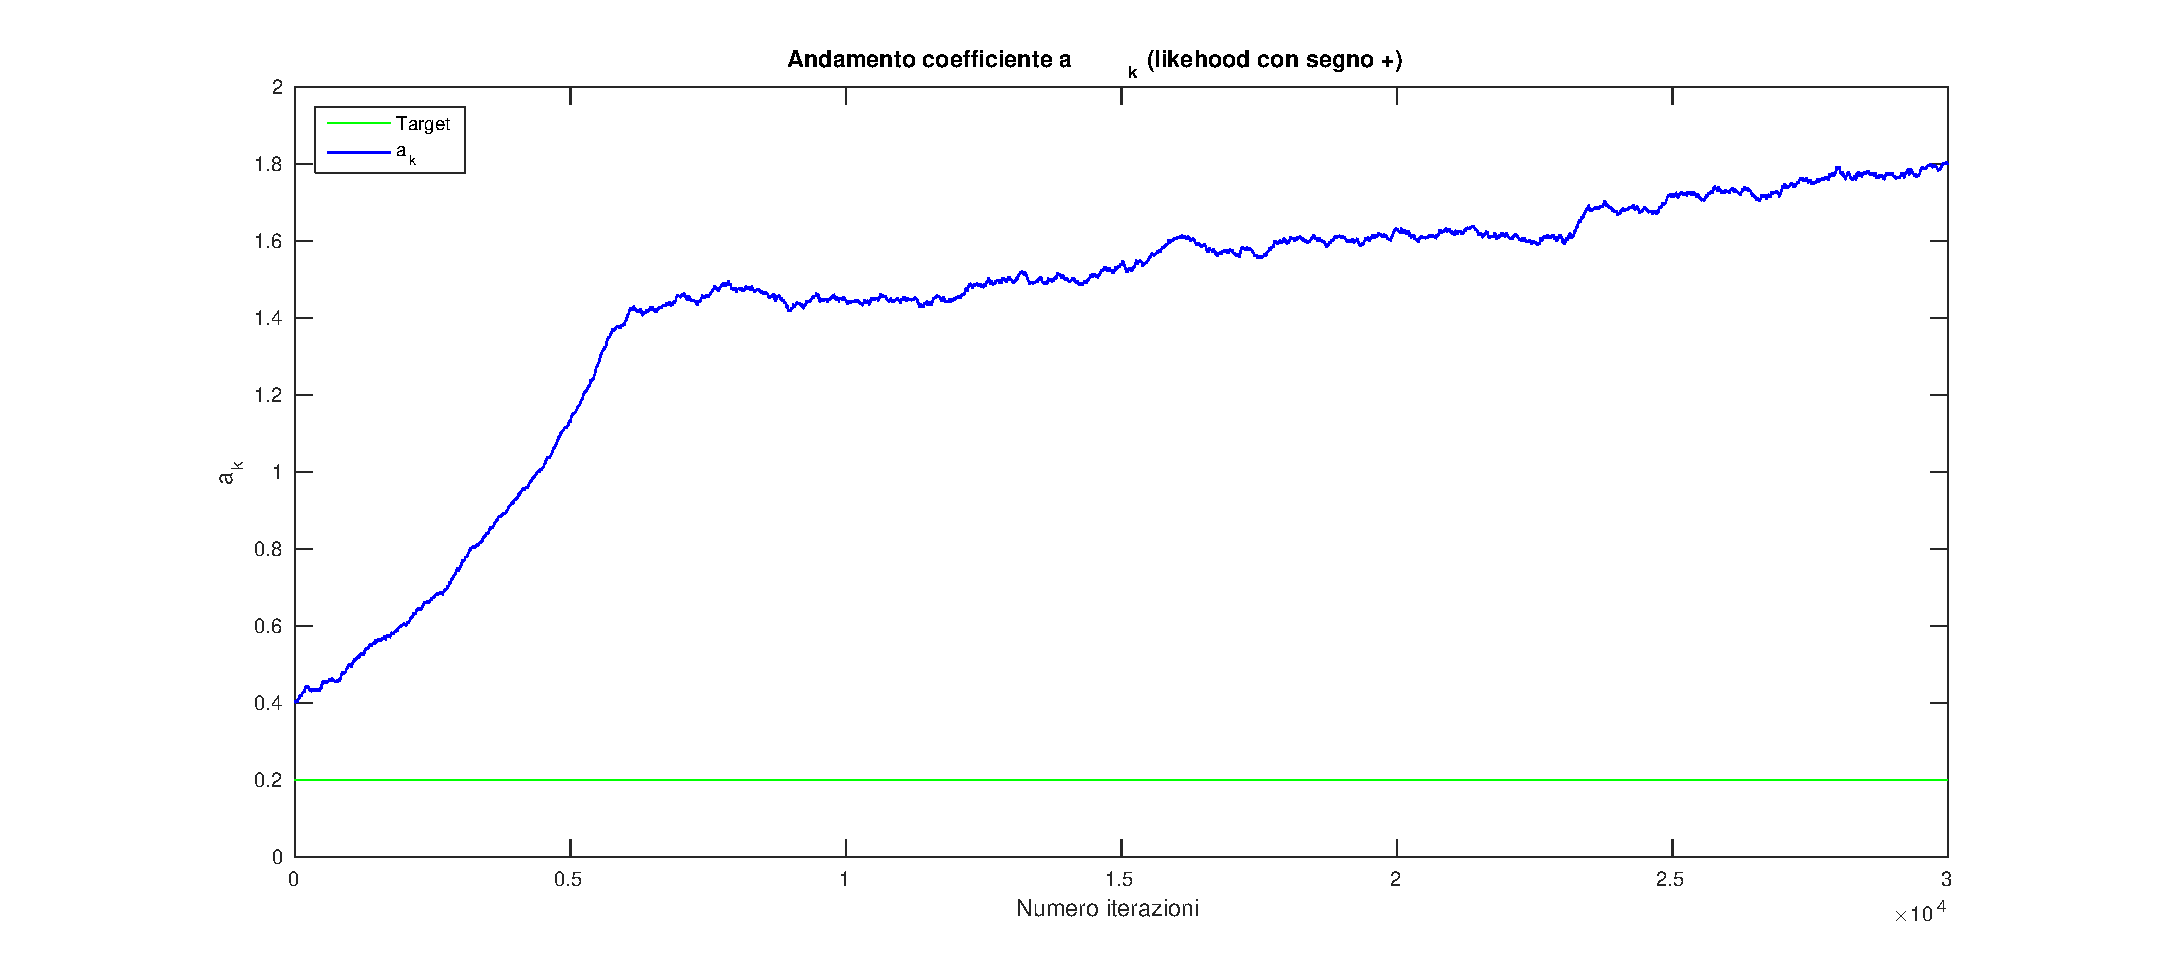
\includegraphics[scale=0.15]{akhplus.eps}
\caption{Serie temporale del coefficiente (segno più)}
\label{fig:minipage1}
\end{minipage}
\quad
\begin{minipage}[b]{0.45\linewidth}
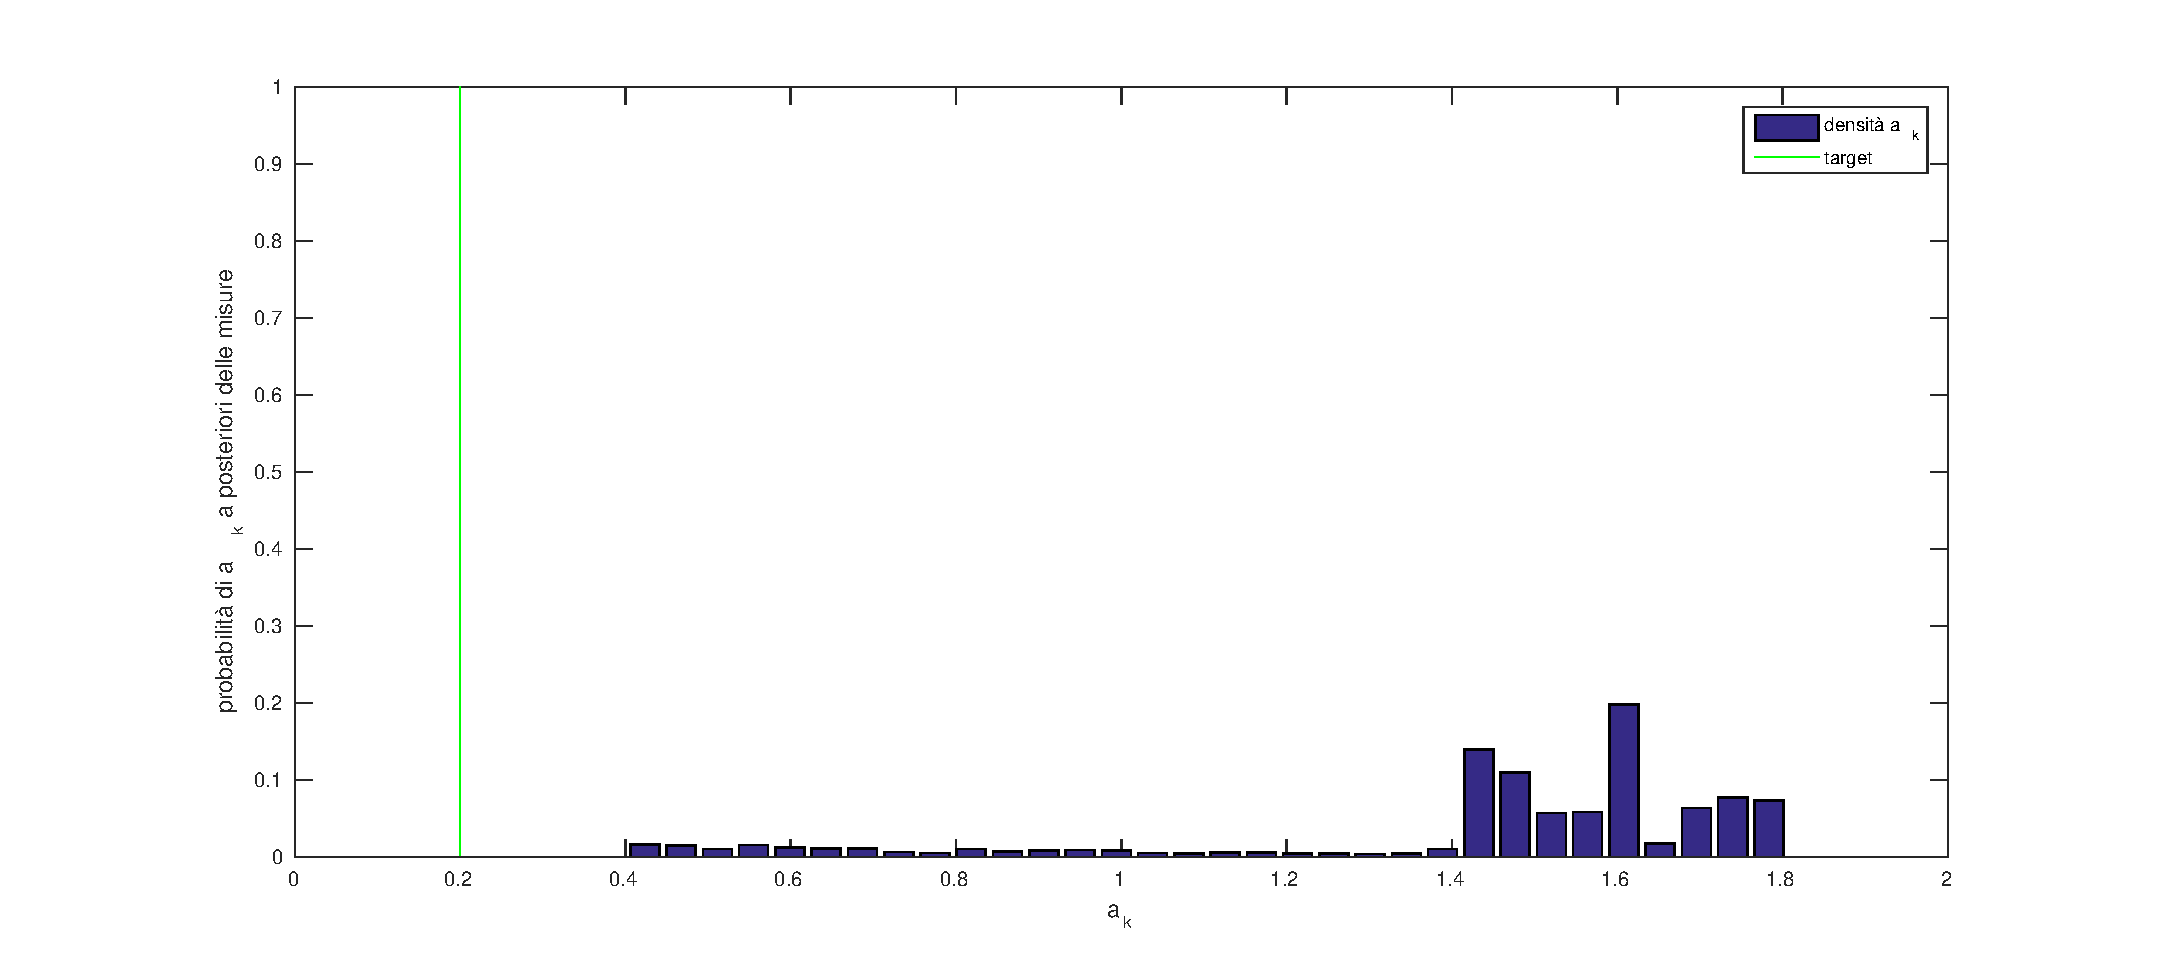
\includegraphics[scale=0.15]{p_ak_plus.eps}
\caption{Ddp a posteriori stimata del coefficiente (segno più)}
\label{fig:minipage2}
\end{minipage}
\end{figure}
\begin{figure}[ht]
\centering
\begin{minipage}[b]{0.45\linewidth}
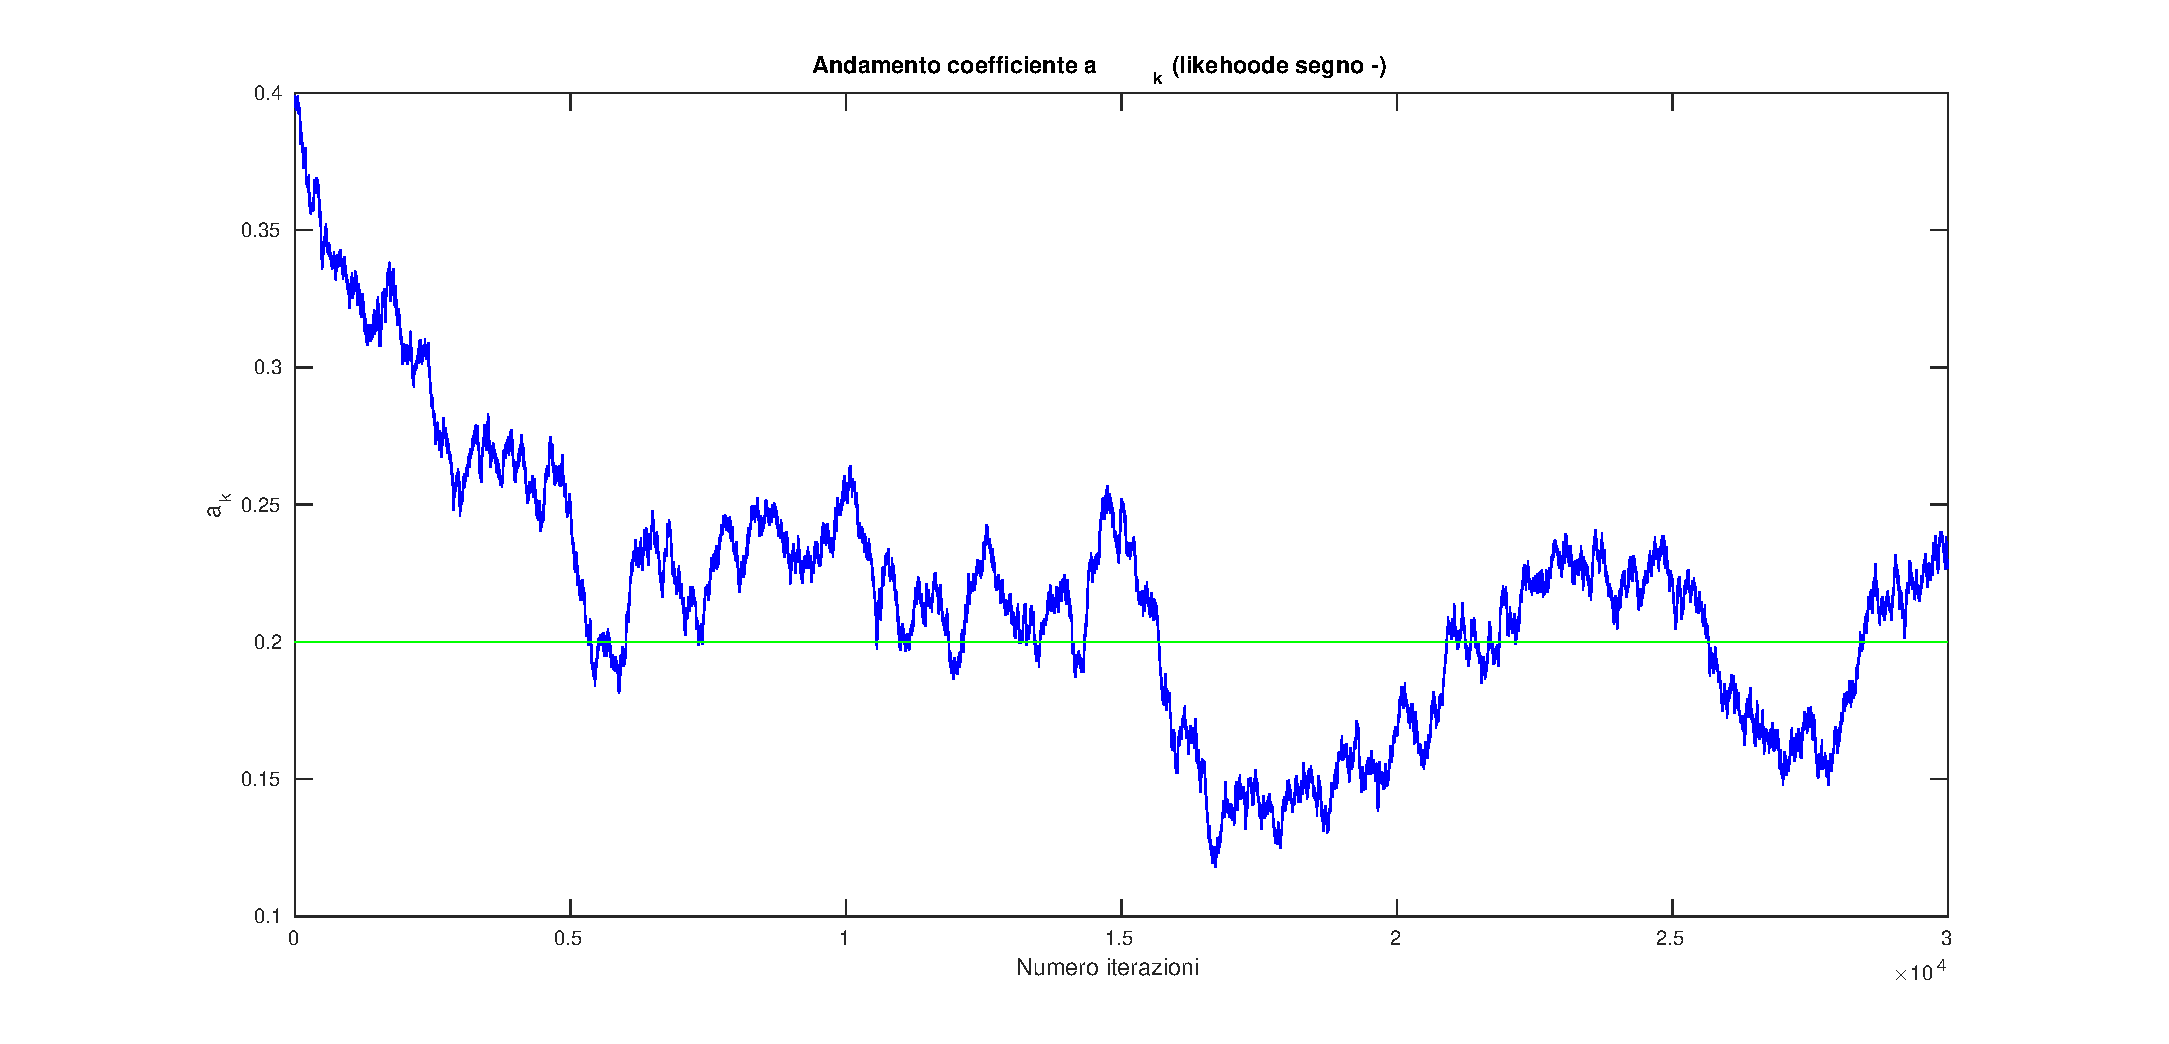
\includegraphics[scale=0.15]{akhminus.eps}
\caption{Serie temporale del coefficiente (segno meno)}
\label{fig:minipage1}
\end{minipage}
\quad
\begin{minipage}[b]{0.45\linewidth}
\includegraphics[scale=0.15]{p_ak_minus.eps}
\caption{Ddp a posteriori stimata del coefficiente (segno meno)}
\label{fig:minipage2}
\end{minipage}
\end{figure}


\section*{Test dell'algoritmo}
In questa sezione vengono mostrati i risultati ottenuti dalla mia implementazione dell'algoritmo nel caso proposto come esempio dall'articolo.\\ \vspace{2em}
L'equazione alle differenze da identificare è
\begin{align*}
y(t)=&0.6y(t-2)-0.5u(t-1)y(t-1)-0.7u(t-2)^2\\
&+0.7u(t-2)^2y(t-2)+0.2e(t-1)^1-0.3u(t-1)e(t-2)+e(t)
\end{align*}
\vspace{2em} \\
I risultati sono riassunti nella seguente tabella, di seguito si entrerà nel dettaglio della spiegazione e dell'analisi dell'esecuzione dell'algoritmo. \vspace{2em} \\
\begin{tabular}{|p{8em}|p{4em}|p{8em}|p{8em}|p{4em}|p{4em}|}
\hline
Termine & Presente  nel target? & Coefficiente Target & Coefficiente identificato & Confidenza & Bin Size\\
\hline
$y(t-2)$ & SI & 0.6 & 0.60404 &  0.7011 & 0.0161 \\ 
\hline
$u(t-1)y(t-1)$ & SI &  -0.5 &  -0.4992  &  0.7925 &   0.0147\\
\hline
$u(t-2)^2$ & SI &  -0.7 &  -0.6939  &  0.2068 &   0.0093\\ 
\hline
$u(t-2)^2y(t-2)$ & SI &   0.7 &   0.7002  &  0.4239  &  0.0113\\ 
\hline
$e(t-1)^1$  & SI &  0.2  &  0.2146  &  0.1403 &   0.0131\\
\hline 
 $u(t-1)^1e(t-2)^1$  & SI & -0.3 &  -0.3383  &  0.0558  &  0.0104\\
\hline 
\end{tabular}
\vspace{2em} \\


Per l'esecuzione sono stati simulati i dati di ingresso e di uscita.\\
Nella costruzione, l'uscita simulata è stata volutamente sporcata dldisturbo bianco.\\
\[u(t)\sim \mathcal{U}(-1,1)\]
\[e(t)\in \normal{0}{\sigma^2_e} \hspace{3em} \sigma_e=0.1\]
Nonostante i segnali siano stati generati con i generatori pseudocasuali di Matlab, è stato verificato 
graficando la funzione di autocorrelazione che essi siano veramente bianchi \\
L'uscita $y(t)$ è stata calcolata applicando ricorsivamente l'equazione alle differenze da identificare.\\
Con tali scelte sono stati ottenuti i seguenti rapporti segnale-rumore
\begin{equation}
SNRu =15.2 dB
\end{equation}
\begin{equation}
SNRy=23.6 dB
\end{equation}
Il setting dei parametri statici e le condizioni iniziali dei parametri dinamici sono i seguenti

\begin{tabular}[t] {|p{10em}|p{0.5\linewidth}|}
\hline
\[lambdaA=2\]
\[lambdaB=2\]
& Valore  atteso iniziale del numero di parametri  \\ \hline

\[sigmaA=5\]
\[sigmaB=5\] &
 Inizializzazione delle varianze delle proposal dei coefficienti\\ \hline
\[c=0.3\] & Rapporto di frequenza tra le mosse dinamiche (morte e nascita) e quella
 di aggiornamento\\ \hline
 \[dynamicOrderP=2 \hspace{1em}\]
\[dynamicOrderN=2 \hspace{1em}\] & Massimo ritardo che compare nei termini disponibili rispettivamente di processo e di rumore.  \\ \hline
\[polinomialOrderP=3\]
\[polinomialOrderN=3\] & Massimo grado polinomiale possibile \\ \hline


\[alphaLA=0.5;\]\[alphaLB=0.5;\]  & Iperparametro di forma \\ \hline


\[betaLA=1.1;\]\[betaLB=1.1;\]  &Iperparametro di scala \\ \hline

\hline
\end{tabular}
\vspace{2em}
\\
Sono state eseguite 30000 iterazioni per studiare l'andamento temporale dell'algoritmo.\\
Tuttavia la convergenza (almeno in termini di struttura del modello) richiede meno iterazioni come si evince dai grafici seguenti 
\begin{figure}[ht]
\quad
\centering
\begin{minipage}[t]{0.45\linewidth}

\includegraphics[width=0.7\textwidth]{modesk.eps} 
\caption{Miglior numero di termini di processo in funzione del numero di iterazioni.   }
\label{fig:minipage1}
\end{minipage}
\quad
\begin{minipage}[t]{0.45\linewidth}
\centering
\includegraphics[width=0.7\textwidth]{BestModelPTransitorio.eps}
\caption{Identificativo del miglior  modello di processo in funzione del numero di iterazioni (Dettaglio del transitorio)}
\label{fig:minipage2}
\end{minipage}
\end{figure}

\begin{figure}[ht]
\quad
\centering
\begin{minipage}[t]{0.45\linewidth}

\includegraphics[width=0.7\textwidth]{modesq.eps} 
\caption{Miglior numero di termini di rumore in funzione del numero di iterazioni.   }
\label{fig:minipage1}
\end{minipage}
\quad
\begin{minipage}[t]{0.45\linewidth}
\centering
\includegraphics[width=0.7\textwidth]{BestModelNTransitorio.eps}
\caption{Identificativo del miglior  modello di rumore in funzione del numero di iterazioni (Dettaglio del transitorio)}
\label{fig:minipage2}
\end{minipage}
\end{figure}
In particolare si ha che l'algoritmo 

\begin{itemize}
\item identifica correttamene il numero di termini di processo $k=4$  in 454 iterazioni
\item identifica correttamene il numero di termini di rumore $q=2$  in 2598 iterazioni
\item identifica correttamene la struttura del modello di processo  in 414 iterazioni
\item identifica correttamene la struttura del modello di rumore  in 93 iterazioni
\end{itemize}
La convergenza dell'algoritmo per quanto riguarda i coefficienti è più difficile da provare in quanto si hanno a disposizione meno iterazioni (quelle in cui la catena è andata a risiedere in un modello con la struttura corretta).\\
Si prenda ad esempio l'andamento del miglior coefficiente $a_2$ nel senso di
\[\arg \max p(a_2|y,P_k,k)\] graficato qui sotto
\begin{center}
\includegraphics[width=0.4\linewidth]{bestcoeffak2eps.eps} 
\end{center}
Si può notare che  dopo 20000 iterazioni si ha ancora una fluttuazione del miglior coefficiente, cosa che potrebbe far dubitare della convergenza. La fluttuazione è però di 0.003 mentre l'ultima dimensione del bin per l'istogramma è 0.017. In realtà tutte le fluttuazioni (da quando la catena risiede per la prima volta nella struttura corretta del modello) sono di entità paragonabile.\\
Si può ritenere dunque che l'algoritmo abbia portato in convergenza il coefficiente al valore\\ $-0.5\pm 0.003$ almeno a partire dall'iterazione 9000 (risultato che conferma la scelta degli autori dell'articolo di fermarsi a 9500 iterazioni)










\begin{figure}[ht]
\quad
\centering
\begin{minipage}[b]{0.45\linewidth}
\centering
\includegraphics[width=0.7\textwidth]{histk.eps} 
\caption{Probabilità a posteriori del numero di termini }
\label{fig:minipage1}
\end{minipage}
\quad
\begin{minipage}[b]{0.45\linewidth}
\centering
\includegraphics[width=0.7\textwidth]{histq.eps}
\caption{Densità di probabilità di $a_2$ a posteriori}
\label{fig:minipage2}
\end{minipage}
\end{figure}


\begin{figure}[ht]
\quad
\centering
\begin{minipage}[b]{0.45\linewidth}
\centering
\includegraphics[width=0.7\textwidth]{ak_1.eps} 
\caption{Densità di probabilità di $a_1$ a posteriori}
\label{fig:minipage1}
\end{minipage}
\quad
\begin{minipage}[b]{0.45\linewidth}
\centering
\includegraphics[width=0.7\textwidth]{ak_2.eps}
\caption{Densità di probabilità di $a_2$ a posteriori}
\label{fig:minipage2}
\end{minipage}
\end{figure}

\begin{figure}[ht]
\centering
\begin{minipage}[b]{0.45\linewidth}
\centering
\includegraphics[width=0.7\textwidth]{ak_3.eps}
\caption{Densità di probabilità di $a_3$ a posteriori}
\label{fig:minipage1}
\end{minipage}
\quad
\begin{minipage}[b]{0.45\linewidth}
\centering
\includegraphics[width=0.7\textwidth]{ak_4.eps}
\caption{Densità di probabilità di $a_4$ a posteriori}
\label{fig:minipage2}
\end{minipage}
\end{figure}


\begin{figure}[ht]
\begin{minipage}[b]{0.45\linewidth}
\centering
\includegraphics[width=0.7\textwidth]{bq_1.eps}
\caption{Densità di probabilità di $b_1$ a posteriori}
\label{fig:minipage1}
\end{minipage}
\quad
\begin{minipage}[b]{0.45\linewidth}
\centering
\includegraphics[width=0.7\textwidth]{bq_2.eps}
\caption{Densità di probabilità di $b_2$ a posteriori}
\label{fig:minipage2}
\end{minipage}\\
\end{figure}


\end{document}
